\label{chapter3}
\chapter{Related work}

Work relating to load profiling can be found in two research verticals or topics. The first one is load profiling and load profile models, which in 
most cases study the load profile curve of the building. Few exceptions study load profiles on appliance-level.
The second vertical is anomaly detection in building energy consumption data. While the first topic is closer, there are quite a few connections with the latter. 
If one wants to do anomaly detection, in some cases, one must first build some kind of "normal consumption profile" 

\section{Load profiling}

Load profiling has been researched since 1980. Load-profiling can be performed in two ways: bottom-up and top-down. 

A bottom-up approach as \cite{SWAN20091819} state "calculates the individual dwelling energy or electricity consumption and extrapolate these results over a target area or region"
Whereas with Top-down approach as \cite{SWAN20091819} state "uses the total energy or electricity consumption estimates to assign them to the characteristics of the building stock"
In other words, Bottom-up sub-meter data, Top-down uses aggregated data. In our case, we take a deeper dive into the bottom-up approach, since it is more relatable.

\cite{Review2021} did a comprehensive review on load profiling. The author defined various load-profile application
subgroups such as demand-side management, planning and control design of energy systems, and residential load profiles. The author also 
grouped modeling techniques as probabilistic models, Markov chains, and Monte Carlo. The author first disclosed the current state of load profiling and issues with past work.
They made a review of existing load profiling models
and asses the-state-of-the art. The review was structured by different methods. Next, they pointed out future research directions
and applications of load profiling models. Finally, the author exposes issues that researchers face and addresses possible solutions with conclusions.

\begin{figure}[h!]
	\centering
	\caption{"Distribution of publications on load profiling from 1985 to 2020. The graph was published by \protect\cite{Review2021}"}
	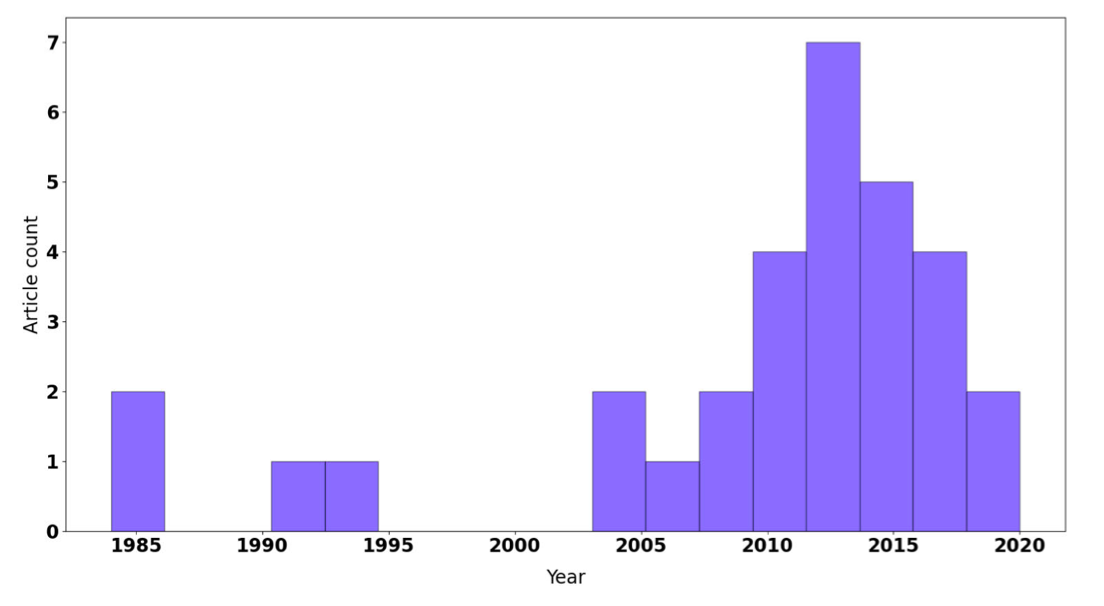
\includegraphics[width=0.9\textwidth]{Figures/publications.png}
	\label{fig:Distribution}
\end{figure}

One of the first publications on load profiling was published by \cite{TRAIN19851103}.
They used a bottom-up approach using sub-meter data and other socioeconomic and demographic characteristics 
to create a load profile or statistically adjusted engineering (SAE) as they call it.
They can adjust the curve based on weather, dwelling size, and income. 
In the same year, \cite{WALKER1985} published a paper where they used a bottom-up approach with psychological factors to create probability models of when will an individual use an appliance.

Since then there were two more in 1995. Research picked up the pace in 2005 with 7 publications in 2013 as figure \ref{fig:Distribution} shows.

\cite{GERBEC2005} tried to assign typical load profiles to a particular group of consumers based on their activity. 
To achieve that, they used probabilistic neural networks as a way of classification. Their methodology was tested in real use scenario. 

\cite{Gao2018} makes use of the bottom-up method to build a forecasting framework for household
load profiling, which takes into account the consumption patterns of residents. 
A model falls into the demand-side management subgroup.
They have developed a "single-day extraction model", designed to select the same days by comparing environmental and household factors, which influence energy consumption.
By using this approach, they have improved the accuracy of predicting behavioral patterns of dwellers. 
This method falls into the probabilistic method subgroup. Results show that their method successfully modeled daily usage.

\cite{Chuan2014} uses load profiling to optimize energy consumption distribution during the day.
This reduces peaks usage and alleviates load off the grid. The author used the bottom-up method, that is, using sum-meter data.
Using this data, he made daily usage analyses on a one-hour basis. Using this information he optimized the daily activation of appliances
so that peaks usage was not as high. Results show that peak shedding was successful. 

\cite{Csoknyai2019} analyzes energy consumption patterns and intervention strategies in residential buildings.
Authors achieve this using a "serious game approach" with a combination of direct user feedback using smart meters. 
The application also provides advice, comparisons, savings, reduction goals, and monitoring.
The approach takes into account almost all dimensions of residential energy usage. Their results show that their serious game was not
able to induce energy-saving behavior.

\cite{Jeong2021} used extreme points in the appliance usage curve to cluster usage profiles.
Usually, the first usage peak is in the morning, and the second one is in the evening. 
Additionally, they used demographic characteristics that are: region, area, age, salary, etc. to improve the results.
Using collected data, they clustered profiles. They had discovered 6 different usage profiles, 
where every cluster had a physical meaning such as energy-saving, morning heavy, evening heavy, etc.

Another clustering methodology was proposed by \cite{Park2019}, using load image profiles and image processing.
They represented time series data as an image. The image is a grid of squares where the y-axis contains monthly data with a resolution of one day,
x-axis contains daily data with a resolution of one hour. Grid if color filled with an algorithm that authors developed,
where red means more activity and blue less. Using digital image filters they transformed the type-1 image to type-2 and from there
used a threshold to obtain type-3. Using that information they clustered data based on images similarly. They used three different 
clustering methods: k-means, FCM, and EM algorithm. Using the Davies-Bouldin index, they were able to prove that image-based clustering performs better than non-image.

\cite{Joana2012} clustered different load profiles using electricity consumption data and surveys. They profiled residential homes. 
They used PCA and k-means resulting in 5 clusters. Similar to other load profiling papers. 

Whereas most of the above-mentioned papers focused on aggregated consumption of building to build a load profile,
authors \cite{Issi2018} focused on appliance-level load profiling.
Their main contribution was to create a realistic per appliance load profile.
They developed a wireless measurement system with smart plugs that enabled them to obtain 
power signatures for each appliance. They evaluated the data and based on observations they determined working cycles for each appliance.
Furthermore, they concluded that 15 \% of consumed power can be shifted, where they took tariffs into account. 

\section{Anomaly detection in building energy consumption data}

A review on Anomaly detection in building energy consumption data was written by \cite{HIMEUR2021116601}.
Here, the authors took a deep dive into detecting anomalies in energy consumption in buildings. 
The author first makes an overview of existing anomaly detection schemes and applications.
Second, they perform a critical analysis and an in-depth discussion of the state-of-the-art.
Next, they describe current trends such as NILM anomaly detection. Finally, they assemble a set of future research directions. 
Both reviews pointed out that NILM anomaly detection or NILM load profiling is a possible future research direction.

\cite{NILMAD2019} authors propose an algorithm
that functions on top of existing state-of-the-art NILM algorithms Hidden Markov model,
combinatorial optimization, Latent Bayesian Modeling, and Graph-based Signal Processing.
They focus on three appliances, a fridge, freezer, and heater. Their metric was the number of operation cycles and energy used within those cycles. 
They implemented sigma variables to represent standard deviation and used rule-based anomaly detection.
So if energy or counts are significantly larger than the mean then the day is considered anomalous.
Their rule had only one manual setting and that was a number of standard deviations before the sample was considered anomalous.
Their results show that sub-meter anomaly detection works decently whereas NILM based anomaly does not work at all. 

\cite{NILMAD22019} published another paper in the same year, where they took a similar approach, except that they used 
only compressor-based appliances such as fridges and air conditioners. They also added a rule to their existing rule-based anomaly 
detection algorithm, but the results still showed that NILM algorithms are not there yet. 

\cite{Castangia2021} used disaggregated sub-meter data to detect anomalies in use consumption.
They used a private dataset of 20 homes from northern Italy with no synthetic anomalies. 
Dataset included data from 2018 to 2020 meaning it included covid induced anomalies. 
The authors first pre-processed the data by aggregating input load in hourly energy consumption, 
the second derived additional features, which are the time of use and duration of the activation.
They use that data to detect single-pint deviations for which they implemented isolation Forest algorithm and
anomalous trends for which to detect, they implemented Change Point Detection. 
